\documentclass{jhwhw}
\usepackage{adjustbox}
\lstset{
  basicstyle=\ttfamily\small, % Small font size for code
  breaklines=true,            % Enable line breaking
  postbreak=\mbox{\textcolor{red}{$\hookrightarrow$}\space}, % Optional: mark where the line was broken
}
\author{Deepak Nathani}
\title{CS292C Homework 2}
\begin{document}
\maketitle

\section{Self-Grade}

\begin{table}[h]
    \centering
    \begin{tabular}{l|c}
        \toprule
        \midrule
        \textbf{Problem} & \textbf{Self-Grade} \\
        \midrule
        {1: Problem Name 1} & {Score} \\
        \midrule
        {2: Problem Name 2} & {Score} \\
        \midrule
        {3: Problem Name 3} & {Score} \\
        \midrule
        {4: Problem Name 4} & {Score} \\
        \midrule
        {5: Problem Name 5} & {Score} \\
        \midrule
        {6: Problem Name 6} & {Score} \\
        \midrule
        {7: Problem Name 7} & {Score} \\
        \midrule
        {8: Problem Name 8} & {Score} \\
        \midrule
        {9: Problem Name 9} & {Score} \\
        \midrule
        {10: Problem Name 10} & {Score} \\
        \midrule
        {11: Problem Name 11} & {Score} \\
        \midrule
        \bottomrule
    \end{tabular}
\end{table}

\section{Problems}
\problem{Install OCaml}
Install OCaml by following the instructions in \texttt{install.md}.
Once you're done, enter \texttt{utop} and evaluate the following expression:
\begin{lstlisting}
print_endline "I have installed OCaml!"
\end{lstlisting}
Include a screenshot of all of \texttt{utop}'s output thus far (including the welcome message) to your PDF file.
\newline
\solution
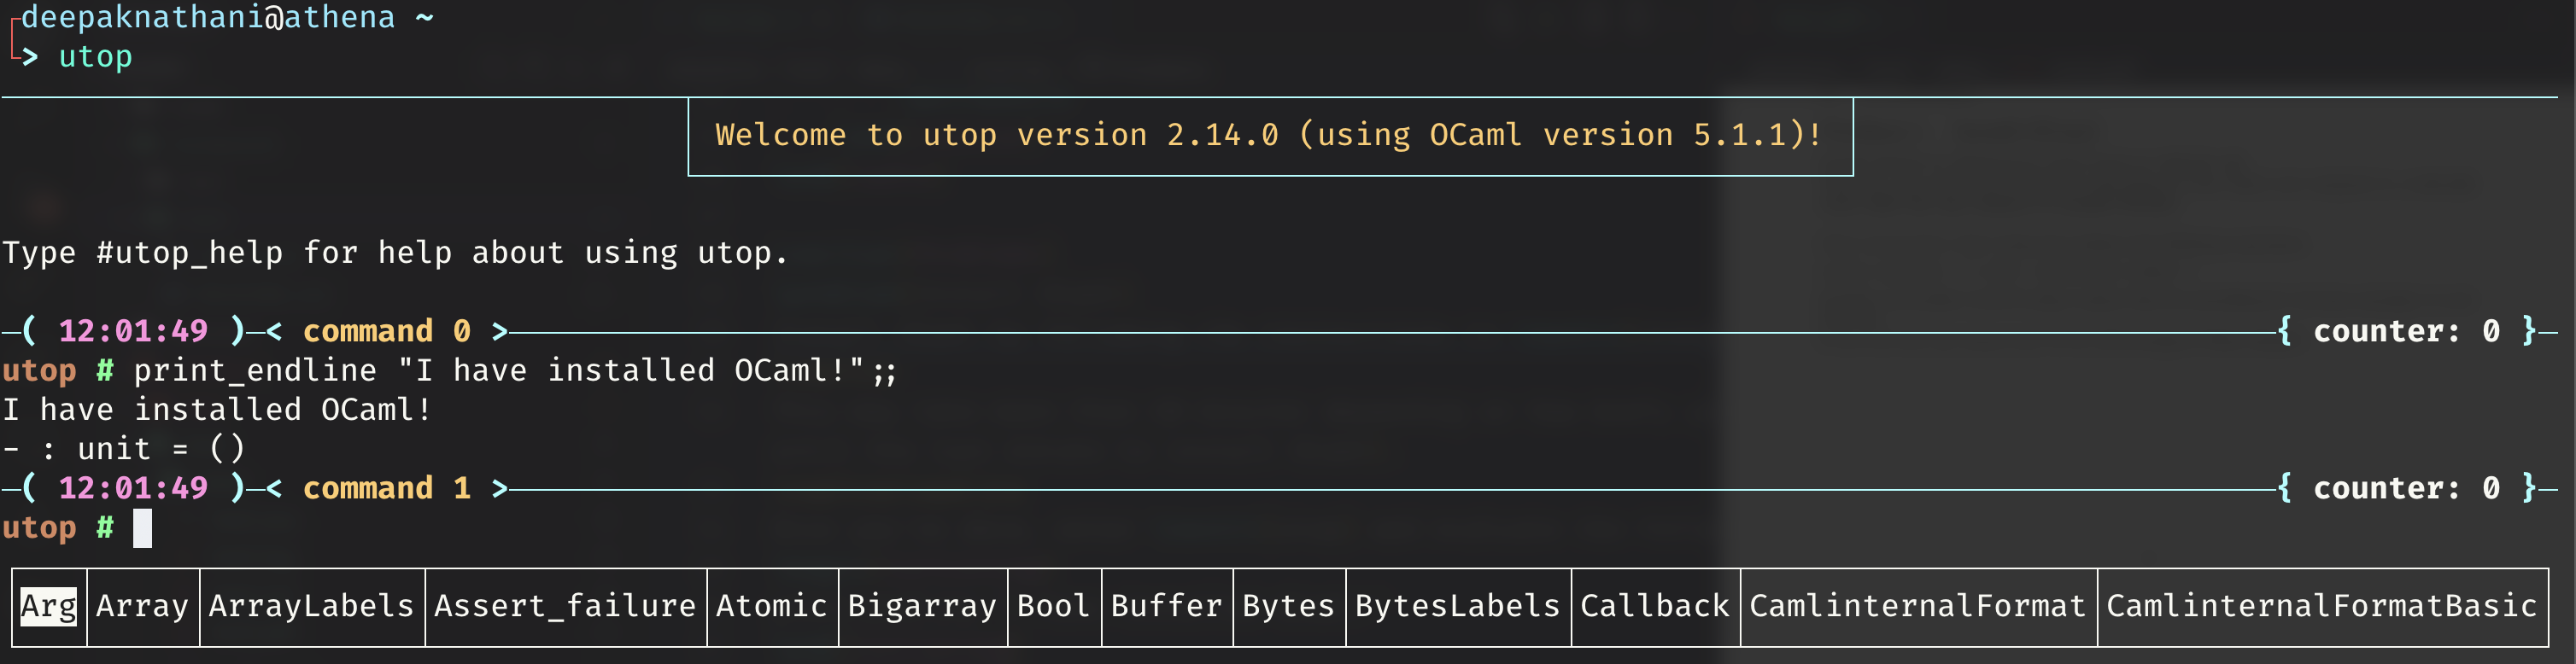
\includegraphics[width=\textwidth]{problem1.png}

\problem{Compress/Duplicate Removal}
\solution
\problem{}
\solution
\problem{}
\solution
\problem{}
\solution
\problem{}
\solution
\problem{}
\solution
\problem{}
\solution
\problem{}
\solution
\problem{}
\solution
\end{document}